\begin{figure}[htbp]
\centering
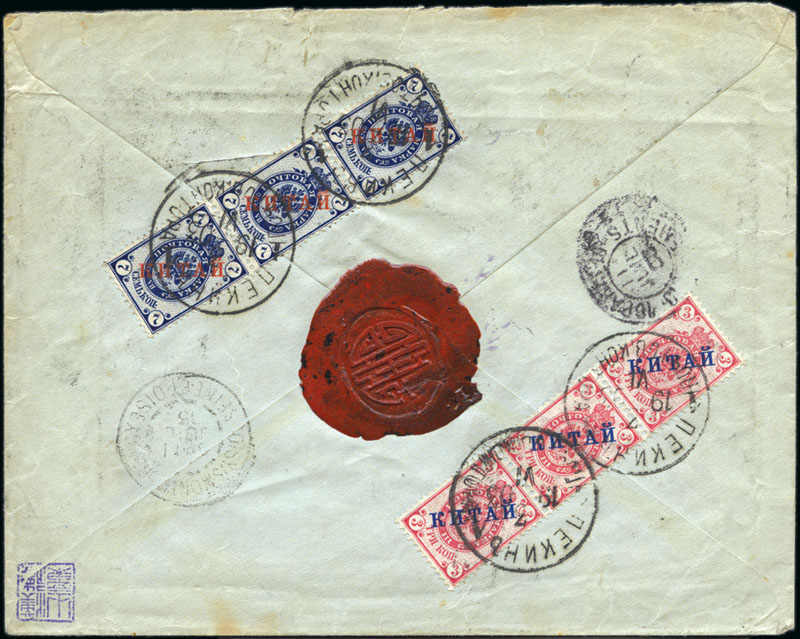
\includegraphics[width=.95\textwidth]{../russian-post-offices-in-china/10032.jpg}
\caption{
10032	PEKING: 1903 Cover registered to France, franked on the reverse with 
"KITAI" 3k and 7k in vertical strips of three, tied by Peking 3.6.03 cds 
(T\&S type 6), registered label on obverse, Paris and Soisy sur Montmorency bs
\euro 300.00 
}  
\end{figure}


\begin{figure}[htbp]
\centering
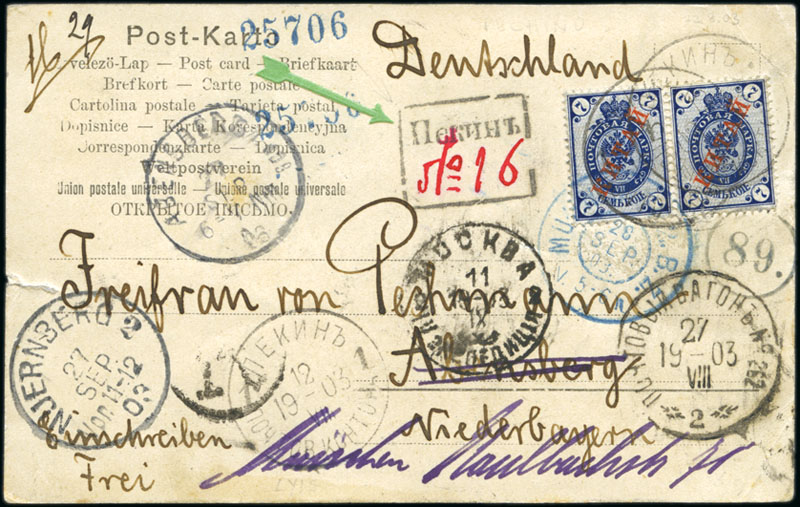
\includegraphics[width=.95\textwidth]{../russian-post-offices-in-china/10033.jpg}
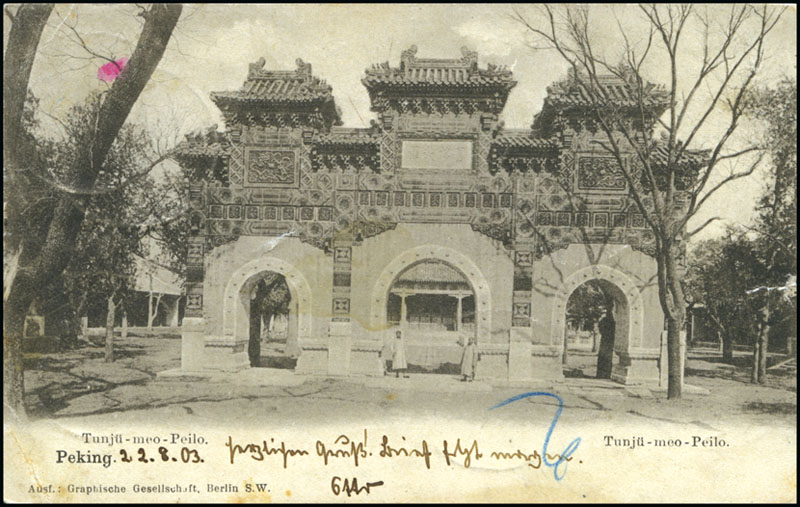
\includegraphics[width=.95\textwidth]{../russian-post-offices-in-china/10033-1.jpg}
\caption{10033 PEKING: 1903 Postcard registered to Germany with "KITAI" 7k pair
tied by Peking 12.8.03 cds (T\&S type 6), with Peking emergency cancel
adjacent (T\&S type 5) modified for use as a registration cachet, with
"Postal Wagon No.262 / 2" transit of the Chinese Eastern Railway, with 
Moscow and German cds, very rare, unusual \& full of character
\euro 800.00
}
\end{figure}

\begin{figure}[htbp]
\centering
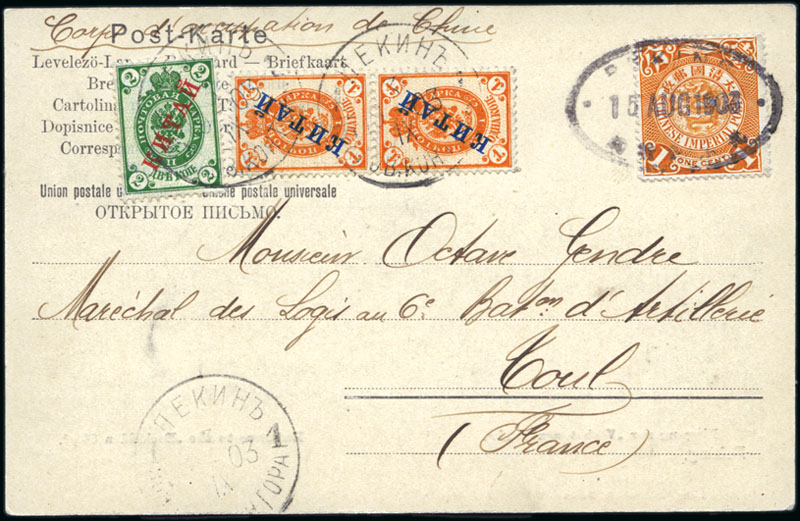
\includegraphics[width=.95\textwidth]{../russian-post-offices-in-china/10034.jpg}
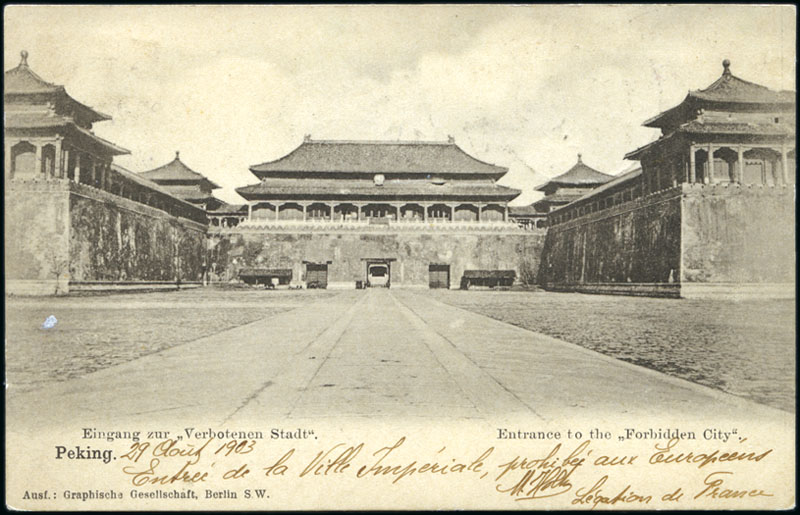
\includegraphics[width=.95\textwidth]{../russian-post-offices-in-china/10034-1.jpg}
\caption{10034		PEKING: 1903 Postcard to France with China 1c Dragon 
tied by Peking bilingual oval ds, further franked with "KITAI" 1k vert. 
pair and 2k tied by Peking 3.9.03 cds (T\&S type 6), a fine philatelic souvenir 
from a member of the French "Boxer" occupying force.
Note: China stamps were only valid for internal use
\euro 300.00 
}
\end{figure} 

\begin{figure}[htbp]
\centering
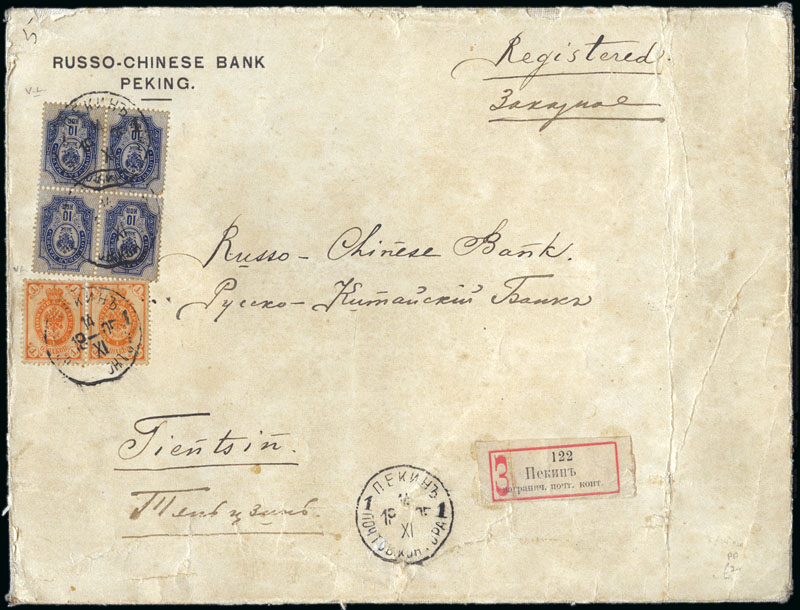
\includegraphics[width=.95\textwidth]{../russian-post-offices-in-china/10035.jpg}
\caption{10035	PEKING: 1905 Large linen envelope from the Russo-Chinese Bank
registered to their office in Tientsin, with ordinary Russian 1k pair and 10k 
block of four tied by Peking 14.11.05 cds (T\&S type 6), reg'd label in 
Cyrillic adjacent, Tientsin arrival, a scarce usage between Russian P.O. in China.
Note: Ordinary Russian stamps were not sold in the Russian P.O.s in Peking
but were accepted if supplied by the customer.
\euro 400.00
}
\end{figure}  

    